% \begin{abstract}
% A computationally-fast inverse design method for nanophotonic structures is presented. The method is based on two complementary convex optimization problems which modify the dielectric structure and resonant field respectively. The design of one- and two-dimensional nanophotonic resonators is demonstrated and is shown to require minimal computational resources.
% \end{abstract}
% 
% \begin{thebibliography}{99}
% \bibitem{Yee66} K. Yee, ``Numerical solution of initial boundary value problems involving Maxwell’s equations in isotropic media,'' IEEE Trans. Antennas Propag. Mag. \textbf{14}, 302-307 (1966).
% \bibitem{AB74} M.~Albani and P.~Bernardi, ``A Numerical Method Based on the Discretization of Maxwell Equations in Integral Form,'' IEEE Trans.~Microwave Theory Tech. \textbf{22}, 446-450 (1974).
% \bibitem{GA79} J.~M.~Gerardy and M.~Ausloos, ``Absorption spectrum of clusters of spheres from the general solution of Maxwell's equations. The long-wavelength limit,'' Phys.~Rev.~B \textbf{22}, 4950-4959 (1979).
% \bibitem{Lon09} P. Deotare, M. McCutcheon, I. Frank, M. Khan, M. Loncar, ``High quality factor photonic crystal nanobeam cavities,'' Appl. Phys. Lett. \textbf{94}, 121106 (2009).
% \bibitem{Sch02} J. Vuckovic, M. Loncar, H. Mabuchi, A. Scherer, ``Design of photonic crystal microcavities for cavity QED,'' Phys. Rev. E \textbf{65}, 1-11 (2002).
% \bibitem{Nod05} Y.~Akahane, T.~Asano, B.~Song, S.~Noda, ``Fine-tuned high-Q photonic-crystal nanocavity,'' Opt. Express \textbf{13}, 1202-1214 (2005).
% \bibitem{Lip08} A. Gondarenko, M. Lipson, ``Low modal volume dipole-like dielectric slab resonator,'' Opt. Express \textbf{16}, 17689-17694 (2008).
% \bibitem{SD05} A. Hakansson, J. Sanchez-Dehesa, ``Inverse designed photonic crystal de-multiplex waveguide coupler,'' Opt. Express \textbf{13}, 5440-5449 (2005).
% \bibitem{Sig04} P. Borel, A. Harpøth, L. Frandsen, M. Kristensen, P. Shi, J. Jensen, and O. Sigmund, ``Topology optimization and fabrication of photonic crystal structures,'' Opt. Express \textbf{12}, 1996-2001 (2004).
% \bibitem{Vuc05} D. Englund, I. Fushman, and J. Vuckovic. ``General Recipe for Designing Photonic Crystal Cavities,'' Opt. Express \textbf{12}, 5961–5975 (2005).
% \bibitem{cholmod} \emph{CHOLMOD} software package, accessed via \emph{Matlab}.
% \bibitem{mycomp} Intel Core 2 Quad $2.5$GHz, 8Gb RAM.
% \bibitem{JJ99} S.~G.~Johnson, J.~D.~Joannopoulos, ``Block-iterative frequency-domain methods for Maxwell’s equations in a planewave basis,'' Opt.~Express \textbf{8}, 967-970 (1999).
% \bibitem{BV04} S. Boyd, L. Vandenberghe, \emph{Convex Optimization} (Cambridge University Press, 2004).
% \bibitem{CVX} M. Grant and S. Boyd, \emph{CVX: Matlab software for disciplined convex programming}, \texttt{http://stanford.edu/$\sim$boyd/cvx}, June 2009.
% \bibitem{Hen06} K. Hennessy, C.~Högerle, E.~Hu, A. Badolato, A. Imamoğlu, ``Tuning photonic nanocavities by atomic force microscope nano-oxidation,'' Appl.~Phys.~Lett.~\textbf{89}, 041118 (2006).
% \bibitem{Aka05} B.~-S.~Song, S.~Noda, T.~Asano, Y.~Akahane, ``Ultra-high-Q photonic double-heterostructure nanocavity,'' Nat. Mater. \textbf{4}, 207-210 (2005).
% \bibitem{Riv09} K.~Rivoire, Z.~Lin, F.~Hatami, W.~Ted Masselink, and J.~Vuckovic, ``Second harmonic generation in gallium phosphide photonic crystal nanocavities with ultralow continuous wave pump power,'' Optics Express \textbf{17}, 22609-22615 (2009).
% \end{thebibliography}
% 
\chapter{Direct design}\label{direct}
% Numerous numerical methods have been devised to solve Maxwell's equations in both time\cite{Yee66} and frequency\cite{AB74,GA79} domains. We refer to these schemes as direct solvers, since they compute the electric and magnetic fields based on current sources, charge distributions and surrounding dielectric and/or metallic structures. While extremely useful in simulating optical components, using direct methods to design optical components, especially in two or three dimensions,  typically requires an extremely time-consuming direct search in a large parameter space\cite{Lon09,Sch02,Nod05,Lip08,SD05}.
% 
% On the other hand, an inverse solver would be much more adept in such design and optimization problems\cite{Sig04,Vuc05}. In this work, we define the inverse problem as that where the electromagnetic field is known, but the surrounding structure is not known. The goal in the inverse problem is, then, to find a dielectric structure that will produce that specific electromagnetic field profile.
% 
% We show that one can design nanophotonic resonators by specifying the electromagnetic field and its desirable characteristics (such as cavity quality (Q) factor and/or mode volume) and then using an inverse solver to find the corresponding dielectric structure. We show that the inverse method used is not only computationally-fast, but is also able to optimize for multiple device characteristics and produce multiple resonances, both of which are very difficult using direct methods. 
% 

\section{Problem formulation}
This work was originally sparked by the realization that 
    the electromagnetic wave equation was not only linear in the field variable,
    but also in the structure variable.
Specifically, that
    \BE \nabla \times \mu_0^{-1} \nabla \times E - \omega^2 \epsilon E = 
        -i\omega J \label{p1:wave} \EE
    is \emph{bi-linear} in both $E$ and $\epsilon$.

We now make the following substitution in order to represent \eq{p1:wave}
    in linear algebra notation:
    \BI $E \to x$, 
    \I  $\epsilon \to z$,
    \I  $\nabla\times\mu_0^{-1}\nabla\times - \omega^2 \epsilon \to A(z)$, and
    \I  $-i\omega J \to b$. \EI
The electromagnetic wave equation (\eq{p1:wave}) can now be expressed simply as
    \BE A(z)x = b, \label{p1:axb} \EE
    which is not only linear in $x$, but also in $z$, 
    since $A(z)$ is linear with respect to $z$.

The linearity of the electromagnetic wave equation with respect to
    the structure variable suggests the following direct design method:
    \begin{enumerate}
    \item choose the electromagnetic field you wish the structure to produce, and
    \item solve the electromagnetic wave equation for the structure variable. 
    \end{enumerate}

In the language of physics, this amounts to computing
    \BE \epsilon = (\nabla\times\mu_0^{-1}\nabla\times E + 
        i \omega J)/ \omega^2 E \EE
    given $E$. 

In the language of linear algebra, we have formulated the following problem:
    \BE \minimize_z \|A(z)x - b\|^2. \label{p1:problem}\EE
    
\section{Implementation}
To solve \eq{p1:axb} numerically, $x$ (field) and $z$ (structure) variables
    are discretized in space using the standard Yee cell 
    used in finite difference methods\cite{Yee66}. 
The matrix $A(z)$ is contructed in Matlab and solved using 
    the standard built-in function.
Because this implementation was only in 1D,
    all the computation needed to perform the direct design
    was completed in under one second 
    on a standard desktop computer.

For verification purposes, 
    a finite-difference time-domain (FDTD) solver was used 
    to obtain the actual field produced by the structure and 
    to verify the accuracy of the design.  

\section{Results}
We now solve \eq{p1:problem} to design nanophotonic resonators in 1D\cite{Lu10}.
We use the magnetic field formulation of the electromagnetic equation
    in the following examples;
    analogous results for the original $E$-field formulation (\eq{p1:wave})
    are expected.

The chosen value for the $x$ (field) is a canonical resonator field; 
    a sinusoid in a Gaussian envelope.
As the result in fig.~\ref{p1:direct} shows,
    the direct method is able to perfectly reproduce the target field;
    however, the resulting structure features
    periodic singularities which render it unmanufacturable.

\begin{figure}[htbp]\centering
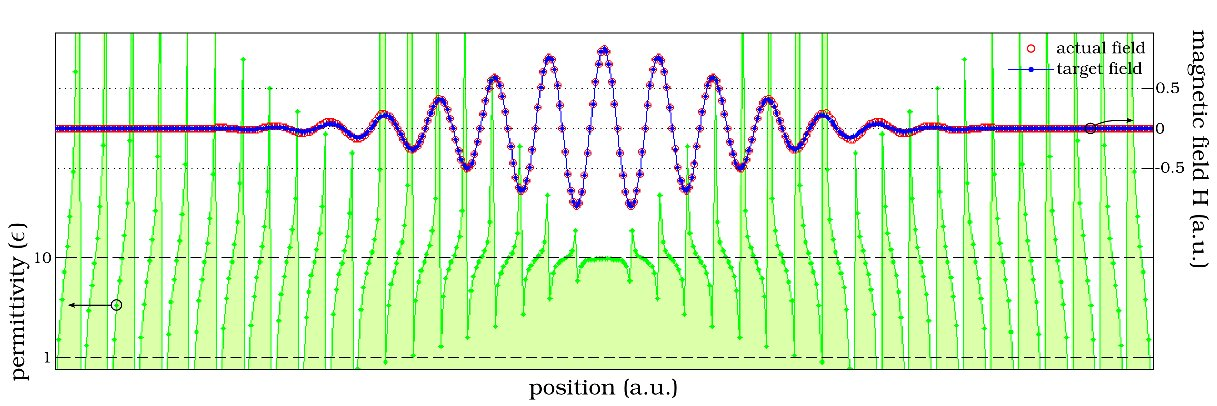
\includegraphics[width=\textwidth]{p1/leastsquares}
\caption{Design of a one-dimensional structure using the direct design method.
    The target field is a sinusoid within a Gaussian envelope. 
    The computed dielectric structure (green area) supports 
        a field (red circles) that exactly matches the target field (blue line). 
    The entire design process is extremely fast and takes less than 
        $1$ second to complete on a generic desktop computer.
    Unfortunately, the periodic singularities in the dielectric structure 
        mean that such a structure is unrealizable in practice.}
\label{p1:direct}\end{figure}

\chapter{Regularized direct design}\label{regularized}
\section{Problem formulation}
The simplest way to produce a well-behaved dielectric structure is 
    to add a regularization term to our direct formulation (\eq{p1:axb}),
    \BE \minimize_z \|A(z)x - b\|^2 + \eta \|z - z_0\|^2. \label{reg:problem}\EE
Here, the regularization term $\eta \|z - z_0\|^2$
    serves to keep $z$ from straying too far from $z_0$, which we choose.
The coefficient $\eta$, then, serves as a knob to control the
    strength of the regularization term.

\section{Implementation}
\Eq{reg:problem} can still be computed in one step
    since the regularization term does not add any computational complexity.
Thus the implementation is only a slight modification
    from that of chapter~\ref{direct}.

\section{Results}
We chose to constrain the values of $z$ ($\epsilon$) 
    around a constant value of $z_0, \epsilon_0 = 10$ and 
    solved \eq{reg:problem} for $\eta=10^{-8}$, $10^{-6}$, and $10^{-4}$;
    the results of which are shown in fig.~\ref{regls pic}\cite{Lu10}.
    
Critically, fig.~\ref{regls pic} shows that there seems
    to be an inherent trade-off between 
        constraining the structure ($z$) 
        and accurately reproducing the field ($x$).

\begin{figure}[htbp]\centering
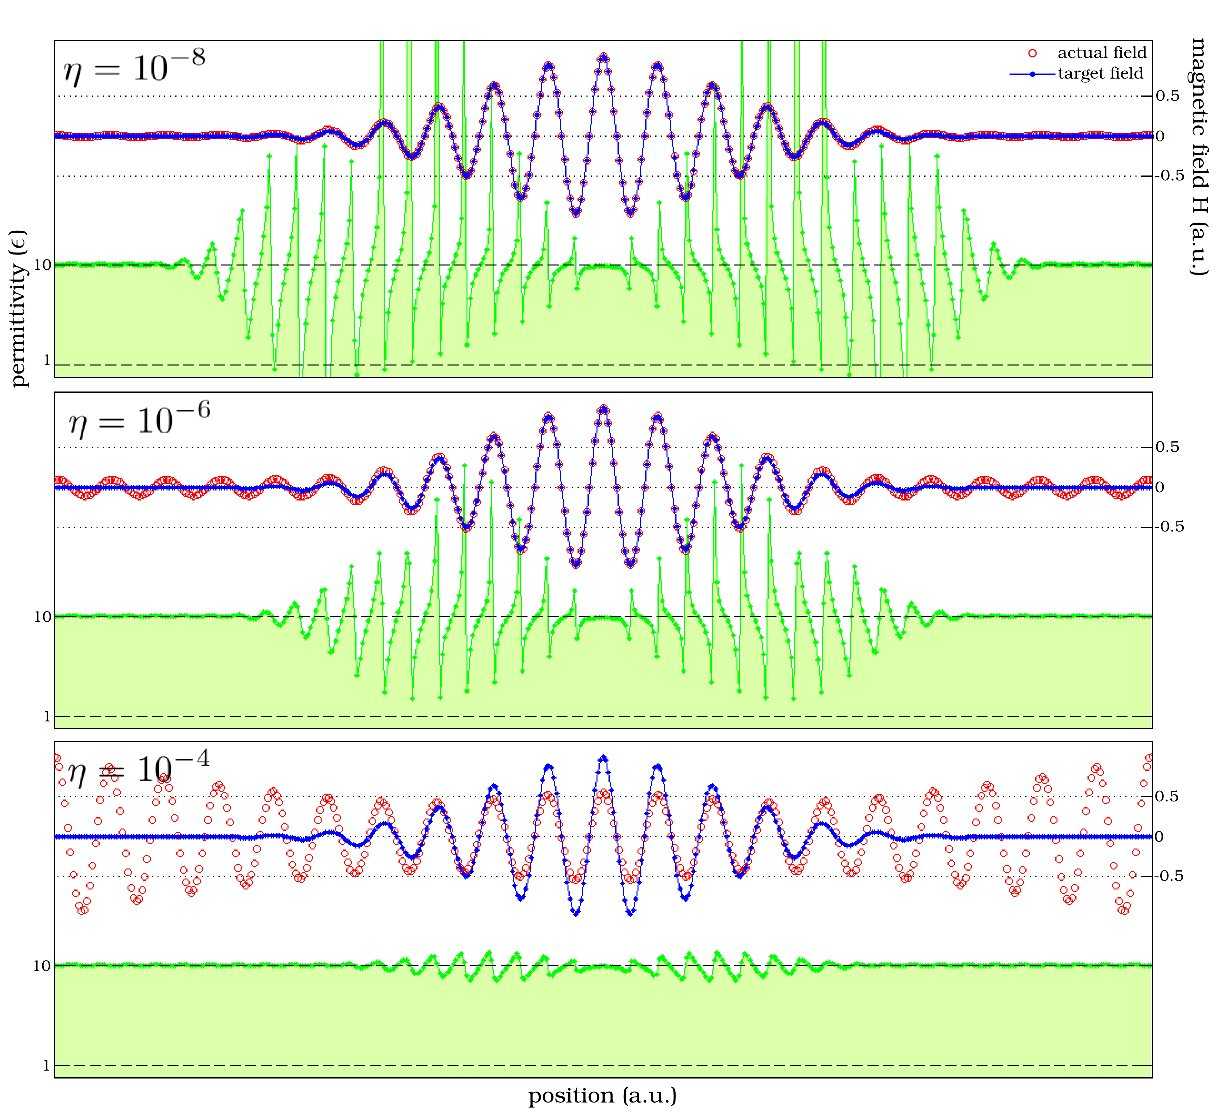
\includegraphics[width=\textwidth]{p1/regularized}
\caption{Regularized design of one-dimensional structures. 
    The same target field is used as in Fig.~\ref{p1:direct}, 
        and the computation time remains below $1$ second. 
    As the regularization parameter, $\eta$, is increased, 
        $\epsilon$ is increasingly constrained to 
        a chosen constant value of $10$. 
    At the same time, the mismatch between target and actual fields 
        increases markedly. 
    This illustrates the apparent trade-off between 
        producing reasonable structures and 
        accurately reproducing a fixed target field.}
\label{regls pic}
\end{figure}




